% ============================================================================
% EMCH 501: Engineering Analysis I - Assignment 4
% ============================================================================

\documentclass[12pt]{article}

% ============================================================================
% PACKAGE IMPORTS
% ============================================================================
\usepackage{amsmath}
\usepackage{graphicx}
\usepackage{amssymb}
\usepackage{tikz}
\usepackage[margin=1in]{geometry}
\usepackage{setspace}
\usepackage{xcolor}
\usepackage{enumitem}
\usepackage{tcolorbox}
\usepackage{fancyhdr}
\usepackage{lastpage}
\usepackage{booktabs}
\usepackage{array}
\usepackage{colortbl}
\usepackage{pgfplots}
\usepackage{listings}
\pgfplotsset{compat=1.18}

% ============================================================================
% HEADER AND FOOTER SETUP
% ============================================================================
\pagestyle{fancy}
\setlength{\headheight}{14.5pt}
\fancyhf{}

\fancyhead[L]{Page \thepage\ of \pageref{LastPage}}
\fancyhead[C]{EMCH 501}
\fancyhead[R]{JC Vaught}

\renewcommand{\headrulewidth}{0pt}

% ============================================================================
% TIKZ LIBRARIES
% ============================================================================
\usetikzlibrary{shapes.geometric, arrows.meta, positioning, decorations.pathmorphing, patterns}

% --- USC Brand Colors ---
\definecolor{USC_Garnet}{HTML}{73000A}
\definecolor{USC_Sandstorm}{HTML}{FFF2E3}
\definecolor{USC_Black90}{HTML}{565656}
\definecolor{USC_Black10}{HTML}{ECECEC}
\definecolor{USC_Honeycomb}{HTML}{65780B}
\definecolor{tablegreen}{RGB}{230,242,230}

% ============================================================================
% CUSTOM COLORED BOXES
% ============================================================================
\newtcolorbox{stepbox}{
  colback=white,
  colframe=USC_Garnet,
  fonttitle=\bfseries,
  title=Step,
  sharp corners,
  colbacktitle=USC_Garnet,
  coltitle=white,
}

\newtcolorbox{codebox}{
  colback=USC_Black10,
  colframe=USC_Black90,
  fonttitle=\bfseries,
  title=Python Implementation,
  sharp corners,
  colbacktitle=USC_Black90,
  coltitle=white,
}

\newtcolorbox{resultsbox}{
  colback=white,
  colframe=USC_Honeycomb,
  fonttitle=\bfseries,
  title=Results,
  sharp corners,
  colbacktitle=USC_Honeycomb,
  coltitle=white,
}

% ============================================================================
% CUSTOM QUESTION AND PART COMMANDS
% ============================================================================
\newcommand{\question}[1]{%
  \clearpage
  \vspace{0.5cm}
  {\noindent\normalsize \textbf{#1}}
  \vspace{0.2cm}
  \hrule
  \vspace{0.1cm}
  \hrule
  \vspace{0.3cm}
}

\newcommand{\questionpart}[1]{%
  \clearpage
  \vspace{0.5cm}
  {\noindent\normalsize \textbf{#1}}
  \vspace{0.2cm}
  \hrule
  \vspace{0.1cm}
  \hrule
  \vspace{0.3cm}
}

% Code listing style
\lstset{
    language=Python,
    basicstyle=\ttfamily\small,
    keywordstyle=\color{blue},
    commentstyle=\color{USC_Honeycomb},
    stringstyle=\color{USC_Garnet},
    breaklines=true,
    showstringspaces=false,
    backgroundcolor=\color{USC_Black10}
}

% ============================================================================
% DOCUMENT INFORMATION
% ============================================================================

\title{EMCH 501: Engineering Analysis I \\ Assignment 4}
\author{Instructor: Yi Wang, Department of Mechanical Engineering \\ University of South Carolina}
\date{Due: December 8, 2025}

% ============================================================================
% BEGIN DOCUMENT
% ============================================================================

\begin{document}

\maketitle
\setlength{\parindent}{0pt}

\setlist[enumerate,1]{label=\arabic*.}
\setlist[enumerate,2]{label=(\alph*)}

% ============================================================================
% TABLE OF CONTENTS
% ============================================================================

\begin{center}
\begin{tcolorbox}[colback=white, colframe=gray!50!black, colbacktitle=gray!20!white,
                  coltitle=black, sharp corners, boxrule=1pt,
                  title=\Large\bfseries Table of Contents]
\begin{tabular}{p{0.82\textwidth}r}
\textbf{Exercise 15.1: Problem 7 (25 pts)} & \\
\quad Part (a): Derivation of Difference Equation \dotfill & \textbf{\pageref{quest:1a}} \\
\quad Part (b): Solution of Poisson Equation \dotfill & \textbf{\pageref{quest:1b}} \\[0.3em]
\textbf{Exercise 15.2: Problem 10 (20 pts)} & \\
\quad Part (a): Finding $\lambda$ \dotfill & \textbf{\pageref{quest:2a}} \\
\quad Part (b): System of Equations \dotfill & \textbf{\pageref{quest:2b}} \\
\quad Part (c): Solving the System \dotfill & \textbf{\pageref{quest:2c}} \\[0.3em]
\textbf{Exercise 15.2: Problem 12 (25 pts)} \dotfill & \textbf{\pageref{quest:3}} \\
\end{tabular}
\vspace{0.2cm}
\end{tcolorbox}
\end{center}

\vspace{0.5cm}

% ============================================================================
% PROBLEM 1: Exercise 15.1 Problem 7 - Part (a)
% ============================================================================

\questionpart{Exercise 15.1: Problem 7 --- Part (a) (25 pts)}\label{quest:1a}

The non-homogeneous form of Laplace's equation is known as Poisson's equation:
\[
\frac{\partial^2 u}{\partial x^2} + \frac{\partial^2 u}{\partial y^2} = f(x,y)
\]
Poisson's equation is commonly used to describe systems involving electric potentials (denoted $u(x,y)$), and $f(x,y)$ can be thought of as the charge density.

\vspace{0.3cm}
\textbf{(a)} Show that the difference equation replacement for Poisson's equation is
\[
u_{i+1,j} + u_{i,j+1} + u_{i-1,j} + u_{i,j-1} - 4u_{i,j} = h^2 f(x,y)
\]

\begin{stepbox}
\textbf{Derivation of the Difference Equation}

We use the central difference approximations for second-order partial derivatives. From Taylor series expansion:

For the second derivative with respect to $x$:
\[
\frac{\partial^2 u}{\partial x^2} \approx \frac{u(x+h, y) - 2u(x, y) + u(x-h, y)}{h^2} = \frac{u_{i+1,j} - 2u_{i,j} + u_{i-1,j}}{h^2}
\]

For the second derivative with respect to $y$:
\[
\frac{\partial^2 u}{\partial y^2} \approx \frac{u(x, y+h) - 2u(x, y) + u(x, y-h)}{h^2} = \frac{u_{i,j+1} - 2u_{i,j} + u_{i,j-1}}{h^2}
\]
\end{stepbox}

\begin{stepbox}
Adding these approximations for Poisson's equation $u_{xx} + u_{yy} = f$:
\[
\frac{u_{i+1,j} - 2u_{i,j} + u_{i-1,j}}{h^2} + \frac{u_{i,j+1} - 2u_{i,j} + u_{i,j-1}}{h^2} = f_{i,j}
\]

Multiplying both sides by $h^2$:
\[
u_{i+1,j} - 2u_{i,j} + u_{i-1,j} + u_{i,j+1} - 2u_{i,j} + u_{i,j-1} = h^2 f_{i,j}
\]

Combining like terms:
\[
u_{i+1,j} + u_{i-1,j} + u_{i,j+1} + u_{i,j-1} - 4u_{i,j} = h^2 f_{i,j}
\]
\end{stepbox}

\begin{resultsbox}
The difference equation replacement for Poisson's equation is:
\[
\boxed{u_{i+1,j} + u_{i,j+1} + u_{i-1,j} + u_{i,j-1} - 4u_{i,j} = h^2 f(x,y)}
\]

This is often called the \textbf{five-point stencil} or \textbf{five-point Laplacian} because it uses the value at the center point and its four immediate neighbors (East, West, North, South).
\end{resultsbox}


% ============================================================================
% PROBLEM 1: Exercise 15.1 Problem 7 - Part (b)
% ============================================================================

\questionpart{Exercise 15.1: Problem 7 --- Part (b)}\label{quest:1b}

\textbf{(b)} Use the result in part (a) to approximate the solution of the Poisson equation
\[
\frac{\partial^2 u}{\partial x^2} + \frac{\partial^2 u}{\partial y^2} = -2
\]
at the interior points of the region in Figure 15.1.7. The mesh size is $h = \dfrac{1}{2}$, $u = 1$ at every point along $ABCD$, and $u = 0$ at every point along $DEFGA$. \underline{Use symmetry} and, if necessary, Gauss-Seidel iteration.

\vspace{0.5cm}
\begin{center}
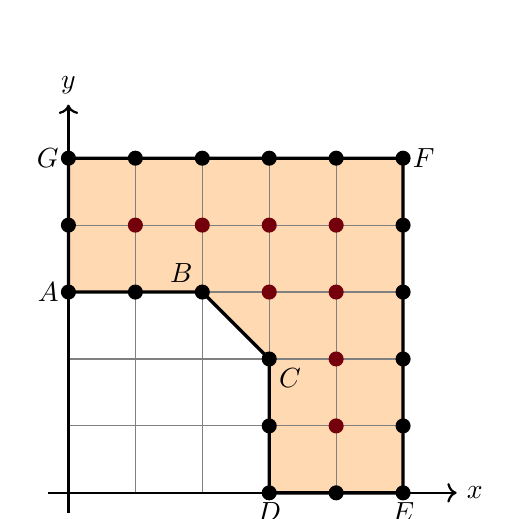
\begin{tikzpicture}[scale=0.85]
    % Fill the L-shaped region
    % Path: (3,0) -> (5,0) -> (5,5) -> (0,5) -> (0,3) -> (2,3) -> (3,2) -> (3,0)
    \fill[orange!30] (3,0) -- (5,0) -- (5,5) -- (0,5) -- (0,3) -- (2,3) -- (3,2) -- cycle;
    
    % Draw grid lines
    \foreach \x in {0,1,2,3,4,5} {
        \draw[gray, thin] (\x, 0) -- (\x, 5);
    }
    \foreach \y in {0,1,2,3,4,5} {
        \draw[gray, thin] (0, \y) -- (5, \y);
    }
    
    % Draw axes
    \draw[->,thick] (-0.3,0) -- (5.8,0) node[right] {$x$};
    \draw[->,thick] (0,-0.3) -- (0,5.8) node[above] {$y$};
    
    % Draw boundary outline (thick black line)
    \draw[very thick] (3,0) -- (5,0) -- (5,5) -- (0,5) -- (0,3) -- (2,3) -- (3,2) -- cycle;
    
    % Interior points (USC Garnet #73000A) - strictly inside the region
    % y=4 row: x = 1, 2, 3, 4
    \foreach \x in {1, 2, 3, 4} {
        \fill[USC_Garnet] (\x, 4) circle (3.2pt);
    }
    % y=3 row: only x = 3, 4 are interior (0,1,2 are on boundary)
    \foreach \x in {3, 4} {
        \fill[USC_Garnet] (\x, 3) circle (3.2pt);
    }
    % y=2 row: only x = 4 is interior
    \fill[USC_Garnet] (4, 2) circle (3.2pt);
    % y=1 row: only x = 4 is interior (3 is on boundary)
    \fill[USC_Garnet] (4, 1) circle (3.2pt);
    
    % Boundary points (black) - all points on the exterior edge
    % Bottom edge: (3,0), (4,0), (5,0)
    \foreach \x in {3, 4, 5} {
        \fill[black] (\x, 0) circle (3.2pt);
    }
    % Right edge: x=5, y = 1,2,3,4,5
    \foreach \y in {1, 2, 3, 4, 5} {
        \fill[black] (5, \y) circle (3.2pt);
    }
    % Top edge: y=5, x = 0,1,2,3,4
    \foreach \x in {0, 1, 2, 3, 4} {
        \fill[black] (\x, 5) circle (3.2pt);
    }
    % Left edge: x=0, y = 3,4
    \foreach \y in {3, 4} {
        \fill[black] (0, \y) circle (3.2pt);
    }
    % Inner boundary horizontal: y=3, x = 1,2
    \foreach \x in {1, 2} {
        \fill[black] (\x, 3) circle (3.2pt);
    }
    % Inner boundary vertical: x=3, y = 1,2
    \foreach \y in {1, 2} {
        \fill[black] (3, \y) circle (3.2pt);
    }
    
    % Labels for boundary corners
    \node[left] at (0, 3) {$A$};
    \node[above left] at (2, 3) {$B$};
    \node[below right] at (3, 2) {$C$};
    \node[below] at (3, 0) {$D$};
    \node[below] at (5, 0) {$E$};
    \node[right] at (5, 5) {$F$};
    \node[left] at (0, 5) {$G$};
    
\end{tikzpicture}

\textbf{FIGURE 15.1.7} Region for Problem 7

\vspace{0.3cm}
\begin{center}
\begin{tabular}{c|c|l}
\toprule
\textbf{Point} & \textbf{Coordinates $(x, y)$} & \textbf{Boundary Condition} \\
\midrule
$A$ & $(0, 3)$ & $u = 1$ (inner boundary) \\
$B$ & $(2, 3)$ & $u = 1$ (inner boundary) \\
$C$ & $(3, 2)$ & $u = 1$ (inner boundary) \\
$D$ & $(3, 0)$ & $u = 0$ (outer boundary) \\
$E$ & $(5, 0)$ & $u = 0$ (outer boundary) \\
$F$ & $(5, 5)$ & $u = 0$ (outer boundary) \\
$G$ & $(0, 5)$ & $u = 0$ (outer boundary) \\
\bottomrule
\end{tabular}
\end{center}

\begin{stepbox}
\textbf{Setting Up the Problem}

For $f(x,y) = -2$ and $h = 1/2$, the difference equation becomes:
\[
u_{i+1,j} + u_{i,j+1} + u_{i-1,j} + u_{i,j-1} - 4u_{i,j} = \left(\frac{1}{2}\right)^2 \cdot (-2) = -\frac{1}{2}
\]

\textbf{Boundary conditions:}
\begin{itemize}
    \item $u = 1$ along $ABCD$ (the stair-step inner boundary)
    \item $u = 0$ along $DEFGA$ (the outer boundary: bottom, right, and top)
\end{itemize}
\end{stepbox}

\begin{stepbox}
\textbf{Identifying Interior Points}

Looking at the grid with $h = 0.5$, the interior points (shown in magenta) are:
\begin{itemize}
    \item Point 1: $(0.5, 1.5)$ --- call this $u_1$
    \item Point 2: $(1.0, 1.5)$ --- call this $u_2$
    \item Point 3: $(1.5, 1.5)$ --- call this $u_3$
    \item Point 4: $(1.0, 1.0)$ --- call this $u_4$
    \item Point 5: $(1.5, 1.0)$ --- call this $u_5$
    \item Point 6: $(1.5, 0.5)$ --- call this $u_6$
\end{itemize}

Due to the diagonal symmetry of the region about the line $y = x$, we have:
\[
u_1 = u_6, \quad u_2 = u_5
\]
This reduces our problem to 4 unknowns: $u_1, u_2, u_3, u_4$.
\end{stepbox}

\begin{stepbox}
\textbf{Writing the Equations}

Using the 5-point stencil: $u_E + u_W + u_N + u_S - 4u_C = -0.5$

\textbf{At $(0.5, 1.5)$, Point 1:}
Neighbors: E=$(1,1.5)=u_2$, W=$(0,1.5)=0$, N=$(0.5,2)=0$, S=$(0.5,1)=1$
\[
u_2 + 0 + 0 + 1 - 4u_1 = -0.5 \implies -4u_1 + u_2 = -1.5
\]

\textbf{At $(1.0, 1.5)$, Point 2:}
Neighbors: E=$(1.5,1.5)=u_3$, W=$(0.5,1.5)=u_1$, N=$(1,2)=0$, S=$(1,1)=u_4$
\[
u_3 + u_1 + 0 + u_4 - 4u_2 = -0.5 \implies u_1 - 4u_2 + u_3 + u_4 = -0.5
\]

\textbf{At $(1.5, 1.5)$, Point 3:}
Neighbors: E=$(2,1.5)=0$, W=$(1,1.5)=u_2$, N=$(1.5,2)=0$, S=$(1.5,1)=u_5=u_2$
\[
0 + u_2 + 0 + u_2 - 4u_3 = -0.5 \implies 2u_2 - 4u_3 = -0.5
\]

\textbf{At $(1.0, 1.0)$, Point 4:}
Neighbors: E=$(1.5,1)=u_5=u_2$, W=$(0.5,1)=1$, N=$(1,1.5)=u_2$, S=$(1,0.5)=1$
\[
u_2 + 1 + u_2 + 1 - 4u_4 = -0.5 \implies 2u_2 - 4u_4 = -2.5
\]
\end{stepbox}

\begin{stepbox}
\textbf{The System of Equations}

\begin{align}
-4u_1 + u_2 &= -1.5 \tag{1}\\
u_1 - 4u_2 + u_3 + u_4 &= -0.5 \tag{2}\\
2u_2 - 4u_3 &= -0.5 \tag{3}\\
2u_2 - 4u_4 &= -2.5 \tag{4}
\end{align}

From equation (1): $u_1 = \frac{1.5 + u_2}{4}$

From equation (3): $u_3 = \frac{0.5 + 2u_2}{4} = \frac{0.125 + 0.5u_2}{1}$

From equation (4): $u_4 = \frac{2.5 + 2u_2}{4} = \frac{0.625 + 0.5u_2}{1}$
\end{stepbox}

\begin{stepbox}
\textbf{Solving for $u_2$}

Substituting into equation (2):
\[
\frac{1.5 + u_2}{4} - 4u_2 + \frac{0.5 + 2u_2}{4} + \frac{2.5 + 2u_2}{4} = -0.5
\]

\[
\frac{1.5 + u_2 + 0.5 + 2u_2 + 2.5 + 2u_2}{4} - 4u_2 = -0.5
\]

\[
\frac{4.5 + 5u_2}{4} - 4u_2 = -0.5
\]

\[
4.5 + 5u_2 - 16u_2 = -2
\]

\[
-11u_2 = -6.5 \implies u_2 = \frac{6.5}{11} = \frac{13}{22} \approx 0.5909
\]
\end{stepbox}

\begin{resultsbox}
\textbf{Final Solution:}

\[
u_2 = u_5 = \frac{13}{22} \approx 0.5909
\]

\[
u_1 = u_6 = \frac{1.5 + 13/22}{4} = \frac{33/22 + 13/22}{4} = \frac{46/22}{4} = \frac{46}{88} = \frac{23}{44} \approx 0.5227
\]

\[
u_3 = \frac{0.5 + 2(13/22)}{4} = \frac{11/22 + 26/22}{4} = \frac{37/22}{4} = \frac{37}{88} \approx 0.4205
\]

\[
u_4 = \frac{2.5 + 2(13/22)}{4} = \frac{55/22 + 26/22}{4} = \frac{81/22}{4} = \frac{81}{88} \approx 0.9205
\]

\begin{center}
\begin{tabular}{c|c|c}
\toprule
Point & Location $(x, y)$ & Value $u$ \\
\midrule
$u_1$ & $(0.5, 1.5)$ & $0.5227$ \\
$u_2$ & $(1.0, 1.5)$ & $0.5909$ \\
$u_3$ & $(1.5, 1.5)$ & $0.4205$ \\
$u_4$ & $(1.0, 1.0)$ & $0.9205$ \\
$u_5$ & $(1.5, 1.0)$ & $0.5909$ \\
$u_6$ & $(1.5, 0.5)$ & $0.5227$ \\
\bottomrule
\end{tabular}
\end{center}
\end{resultsbox}

\begin{codebox}
\begin{lstlisting}
import numpy as np

# Set up the system Ax = b
# Variables: [u1, u2, u3, u4]
A = np.array([
    [-4,  1,  0,  0],   # Eq 1: -4u1 + u2 = -1.5
    [ 1, -4,  1,  1],   # Eq 2: u1 - 4u2 + u3 + u4 = -0.5
    [ 0,  2, -4,  0],   # Eq 3: 2u2 - 4u3 = -0.5
    [ 0,  2,  0, -4]    # Eq 4: 2u2 - 4u4 = -2.5
])

b = np.array([-1.5, -0.5, -0.5, -2.5])

# Solve
u = np.linalg.solve(A, b)
print("Solution:")
print(f"u1 = u6 = {u[0]:.4f}")
print(f"u2 = u5 = {u[1]:.4f}")
print(f"u3 = {u[2]:.4f}")
print(f"u4 = {u[3]:.4f}")
\end{lstlisting}
\end{codebox}


% ============================================================================
% PROBLEM 2: Exercise 15.2 Problem 10 - Part (a)
% ============================================================================

\questionpart{Exercise 15.2: Problem 10 --- Part (a) (20 pts)}\label{quest:2a}

Consider the boundary-value problem from Example 2:
\begin{align*}
0.25\frac{\partial^2 u}{\partial x^2} &= \frac{\partial u}{\partial t}, \quad 0 < x < 2, \quad 0 < t < 0.3\\
u(0,t) &= 0, \quad u(2,t) = 0, \quad 0 \leq t \leq 0.3\\
u(x,0) &= \sin(\pi x), \quad 0 \leq x \leq 2
\end{align*}
using $n = 4$, $m = 30$.

\vspace{0.3cm}
\textbf{(a)} Find $\lambda$

\begin{stepbox}
\textbf{Identifying Parameters}

The PDE is $0.25 u_{xx} = u_t$, which can be written as $u_t = k u_{xx}$ where $k = 0.25$ is the thermal diffusivity.

\textbf{Spatial discretization:} With $n = 4$ divisions over $[0, 2]$:
\[
h = \frac{L}{n} = \frac{2}{4} = 0.5
\]

\textbf{Temporal discretization:} With $m = 30$ divisions over $[0, 0.3]$:
\[
\Delta t = \frac{T}{m} = \frac{0.3}{30} = 0.01
\]
\end{stepbox}

\begin{stepbox}
\textbf{Computing $\lambda$}

The stability parameter $\lambda$ for the heat equation is defined as:
\[
\lambda = \frac{k \Delta t}{h^2}
\]

Substituting our values:
\[
\lambda = \frac{0.25 \times 0.01}{(0.5)^2} = \frac{0.0025}{0.25} = 0.01
\]
\end{stepbox}

\begin{resultsbox}
\[
\boxed{\lambda = 0.01}
\]
\end{resultsbox}


% ============================================================================
% PROBLEM 2: Exercise 15.2 Problem 10 - Part (b)
% ============================================================================

\questionpart{Exercise 15.2: Problem 10 --- Part (b)}\label{quest:2b}

\textbf{(b)} Use the Crank-Nicholson difference equation
\[
-u_{i-1,j+1} + \alpha u_{i,j+1} - u_{i+1,j+1} = u_{i+1,j} - \beta u_{i,j} + u_{i-1,j}
\]
(where $\alpha = 2(1 + 1/\lambda)$ and $\beta = 2(1 - 1/\lambda)$, $j = 0, 1, ..., m-1$ and $i = 1, 2, ..., n-1$)

to find the system of equations for $u_{1,1}$, $u_{2,1}$ and $u_{3,1}$ --- that is, the approximate values of $u$ on the first time line. [Hint: Set $j = 0$ and let $i$ take on the values 1,2,3].

\begin{stepbox}
\textbf{Computing $\alpha$ and $\beta$}

With $\lambda = 0.01$:
\[
\alpha = 2\left(1 + \frac{1}{\lambda}\right) = 2\left(1 + \frac{1}{0.01}\right) = 2(1 + 100) = 202
\]
\[
\beta = 2\left(1 - \frac{1}{\lambda}\right) = 2\left(1 - 100\right) = 2(-99) = -198
\]

Note: $-\beta = 198$ (the right-hand side has $-\beta u_{i,j}$, so we get $+198 u_{i,j}$).
\end{stepbox}

\begin{stepbox}
\textbf{Initial Conditions at $j = 0$}

At $t = 0$, $u(x, 0) = \sin(\pi x)$ with $h = 0.5$:
\begin{align*}
u_{0,0} &= \sin(0) = 0 \\
u_{1,0} &= \sin(0.5\pi) = 1 \\
u_{2,0} &= \sin(\pi) = 0 \\
u_{3,0} &= \sin(1.5\pi) = -1 \\
u_{4,0} &= \sin(2\pi) = 0
\end{align*}

\textbf{Boundary conditions:} $u_{0,j} = 0$ and $u_{4,j} = 0$ for all $j$.
\end{stepbox}

\begin{stepbox}
\textbf{Equations at $j = 0$ (First Time Step)}

The Crank-Nicholson equation is:
\[
-u_{i-1,j+1} + 202 u_{i,j+1} - u_{i+1,j+1} = u_{i+1,j} + 198 u_{i,j} + u_{i-1,j}
\]

\textbf{For $i = 1$:}
\begin{align*}
-u_{0,1} + 202u_{1,1} - u_{2,1} &= u_{2,0} + 198u_{1,0} + u_{0,0} \\
-0 + 202u_{1,1} - u_{2,1} &= 0 + 198(1) + 0
\end{align*}
\[
\boxed{202u_{1,1} - u_{2,1} = 198}
\]

\textbf{For $i = 2$:}
\begin{align*}
-u_{1,1} + 202u_{2,1} - u_{3,1} &= u_{3,0} + 198u_{2,0} + u_{1,0} \\
-u_{1,1} + 202u_{2,1} - u_{3,1} &= -1 + 198(0) + 1
\end{align*}
\[
\boxed{-u_{1,1} + 202u_{2,1} - u_{3,1} = 0}
\]

\textbf{For $i = 3$:}
\begin{align*}
-u_{2,1} + 202u_{3,1} - u_{4,1} &= u_{4,0} + 198u_{3,0} + u_{2,0} \\
-u_{2,1} + 202u_{3,1} - 0 &= 0 + 198(-1) + 0
\end{align*}
\[
\boxed{-u_{2,1} + 202u_{3,1} = -198}
\]
\end{stepbox}

\begin{resultsbox}
\textbf{System of Equations:}
\begin{align*}
202u_{1,1} - u_{2,1} &= 198 \\
-u_{1,1} + 202u_{2,1} - u_{3,1} &= 0 \\
-u_{2,1} + 202u_{3,1} &= -198
\end{align*}

In matrix form:
\[
\begin{pmatrix}
202 & -1 & 0 \\
-1 & 202 & -1 \\
0 & -1 & 202
\end{pmatrix}
\begin{pmatrix}
u_{1,1} \\
u_{2,1} \\
u_{3,1}
\end{pmatrix}
=
\begin{pmatrix}
198 \\
0 \\
-198
\end{pmatrix}
\]
\end{resultsbox}


% ============================================================================
% PROBLEM 2: Exercise 15.2 Problem 10 - Part (c)
% ============================================================================

\questionpart{Exercise 15.2: Problem 10 --- Part (c)}\label{quest:2c}

\textbf{(c)} Solve the system of three equations \underline{without} the aid of a computer program. Compare your results with the corresponding entries in Table 15.2.3.

\begin{stepbox}
\textbf{Using Symmetry}

From the initial condition $u(x, 0) = \sin(\pi x)$, we observe that:
\[
\sin(\pi(2-x)) = \sin(2\pi - \pi x) = -\sin(\pi x)
\]

This antisymmetry about $x = 1$ is preserved by the heat equation. Therefore:
\[
u_{1,j} = -u_{3,j} \quad \text{for all } j
\]

Also, at $x = 1$ (the center), $u_{2,j} = 0$ for all $j$ by symmetry.
\end{stepbox}

\begin{stepbox}
\textbf{Solving Using Symmetry}

Let $u_{1,1} = -u_{3,1}$ and $u_{2,1} = 0$.

From equation (1): $202u_{1,1} - u_{2,1} = 198$
\[
202u_{1,1} - 0 = 198 \implies u_{1,1} = \frac{198}{202} = \frac{99}{101}
\]

Therefore:
\[
u_{3,1} = -u_{1,1} = -\frac{99}{101}
\]
\end{stepbox}

\begin{stepbox}
\textbf{Verification}

Check equation (2): $-u_{1,1} + 202u_{2,1} - u_{3,1} = 0$
\[
-\frac{99}{101} + 202(0) - \left(-\frac{99}{101}\right) = -\frac{99}{101} + \frac{99}{101} = 0 \checkmark
\]

Check equation (3): $-u_{2,1} + 202u_{3,1} = -198$
\[
-0 + 202\left(-\frac{99}{101}\right) = -\frac{202 \times 99}{101} = -\frac{2 \times 99}{1} = -198 \checkmark
\]
\end{stepbox}

\begin{resultsbox}
\textbf{Solutions:}
\[
u_{1,1} = \frac{99}{101} \approx 0.9802
\]
\[
u_{2,1} = 0
\]
\[
u_{3,1} = -\frac{99}{101} \approx -0.9802
\]

\textbf{Comparison with Table 15.2.3:}

The table uses a finer mesh ($h = 0.25$) with $x$-values at $0.25, 0.50, 0.75, 1.00, 1.25, 1.50, 1.75$. At $t = 0.05$:
\begin{itemize}
    \item $u(0.50, 0.05) = 0.8894$ (table value with $h = 0.25$)
    \item Our coarser grid ($h = 0.5$) gives $u(0.5, 0.01) \approx 0.9802$
\end{itemize}

The difference is due to:
\begin{enumerate}
    \item Different mesh size ($h = 0.5$ vs $h = 0.25$)
    \item Different time step ($\Delta t = 0.01$ vs the table's parameters)
\end{enumerate}
\end{resultsbox}

\vspace{0.5cm}
\begin{center}
\textbf{TABLE 15.2.3} \quad Crank-Nicholson Method with $h = 0.25$, $k = 0.01$, $\lambda = 0.25$

\vspace{0.3cm}
\begin{tabular}{c|ccccccc}
\toprule
Time & $x = 0.25$ & $x = 0.50$ & $x = 0.75$ & $x = 1.00$ & $x = 1.25$ & $x = 1.50$ & $x = 1.75$ \\
\midrule
\rowcolor{tablegreen} 0.00 & 0.7071 & 1.0000 & 0.7071 & 0.0000 & $-0.7071$ & $-1.0000$ & $-0.7071$ \\
0.05 & 0.6289 & 0.8894 & 0.6289 & 0.0000 & $-0.6289$ & $-0.8894$ & $-0.6289$ \\
\rowcolor{tablegreen} 0.10 & 0.5594 & 0.7911 & 0.5594 & 0.0000 & $-0.5594$ & $-0.7911$ & $-0.5594$ \\
0.15 & 0.4975 & 0.7036 & 0.4975 & 0.0000 & $-0.4975$ & $-0.7036$ & $-0.4975$ \\
\rowcolor{tablegreen} 0.20 & 0.4425 & 0.6258 & 0.4425 & 0.0000 & $-0.4425$ & $-0.6258$ & $-0.4425$ \\
0.25 & 0.3936 & 0.5567 & 0.3936 & 0.0000 & $-0.3936$ & $-0.5567$ & $-0.3936$ \\
\rowcolor{tablegreen} 0.30 & 0.3501 & 0.4951 & 0.3501 & 0.0000 & $-0.3501$ & $-0.4951$ & $-0.3501$ \\
\bottomrule
\end{tabular}
\end{center}


% ============================================================================
% PROBLEM 3: Exercise 15.2 Problem 12
% ============================================================================

\questionpart{Exercise 15.2: Problem 12 (25 pts)}\label{quest:3}

Use the difference equation
\[
u_{i,j+1} = \lambda u_{i+1,j} + (1 - 2\lambda)u_{i,j} + \lambda u_{i-1,j}
\]
to approximate the solution of the boundary-value problem
\begin{align*}
\frac{\partial^2 u}{\partial x^2} &= \frac{\partial u}{\partial t}, \quad 0 < x < 1, \quad 0 < t < 1\\
u(0,t) &= 0, \quad u(1,t) = 0, \quad 0 \leq t \leq 1\\
u(x,0) &= x(1-x), \quad 0 \leq x \leq 1
\end{align*}

Use $n = 5$ and $m = 50$. \textbf{Solve this using Matlab, Python, or another programming language.}

\begin{stepbox}
\textbf{Step 1: Determine Grid Parameters}

\textbf{Spatial discretization:} With $n = 5$ divisions over $[0, 1]$:
\[
h = \frac{1}{n} = \frac{1}{5} = 0.2
\]

\textbf{Temporal discretization:} With $m = 50$ divisions over $[0, 1]$:
\[
\Delta t = \frac{1}{m} = \frac{1}{50} = 0.02
\]

For the heat equation $u_t = u_{xx}$ (diffusivity $k = 1$):
\[
\lambda = \frac{k \Delta t}{h^2} = \frac{1 \times 0.02}{(0.2)^2} = \frac{0.02}{0.04} = 0.5
\]

\textbf{Stability:} The explicit method is stable when $\lambda \leq 0.5$. We are exactly at the stability limit.
\end{stepbox}

\begin{stepbox}
\textbf{Step 2: Initial and Boundary Conditions}

\textbf{Initial condition} at $t = 0$: $u(x, 0) = x(1-x)$

Grid points $x_i = ih$ for $i = 0, 1, 2, 3, 4, 5$:
\begin{center}
\begin{tabular}{c|cccccc}
$i$ & 0 & 1 & 2 & 3 & 4 & 5 \\
\hline
$x_i$ & 0 & 0.2 & 0.4 & 0.6 & 0.8 & 1.0 \\
$u_{i,0}$ & 0 & 0.16 & 0.24 & 0.24 & 0.16 & 0
\end{tabular}
\end{center}

\textbf{Boundary conditions:} $u_{0,j} = 0$ and $u_{5,j} = 0$ for all $j$.
\end{stepbox}

\begin{stepbox}
\textbf{Step 3: The Explicit Update Formula}

With $\lambda = 0.5$, the difference equation simplifies to:
\[
u_{i,j+1} = 0.5 \cdot u_{i+1,j} + (1 - 1) \cdot u_{i,j} + 0.5 \cdot u_{i-1,j}
\]
\[
u_{i,j+1} = \frac{1}{2}(u_{i+1,j} + u_{i-1,j})
\]

This is simply the \textbf{average of the neighboring values}!
\end{stepbox}

\begin{stepbox}
\textbf{Step 4: First Few Time Steps (Manual)}

\textbf{$j = 0 \to j = 1$:}
\begin{align*}
u_{1,1} &= 0.5(u_{2,0} + u_{0,0}) = 0.5(0.24 + 0) = 0.12\\
u_{2,1} &= 0.5(u_{3,0} + u_{1,0}) = 0.5(0.24 + 0.16) = 0.20\\
u_{3,1} &= 0.5(u_{4,0} + u_{2,0}) = 0.5(0.16 + 0.24) = 0.20\\
u_{4,1} &= 0.5(u_{5,0} + u_{3,0}) = 0.5(0 + 0.24) = 0.12
\end{align*}

\textbf{$j = 1 \to j = 2$:}
\begin{align*}
u_{1,2} &= 0.5(0.20 + 0) = 0.10\\
u_{2,2} &= 0.5(0.20 + 0.12) = 0.16\\
u_{3,2} &= 0.5(0.12 + 0.20) = 0.16\\
u_{4,2} &= 0.5(0 + 0.20) = 0.10
\end{align*}
\end{stepbox}

\begin{codebox}
\begin{lstlisting}
import numpy as np
import matplotlib.pyplot as plt

# Parameters
L = 1.0; T_final = 1.0
n = 5; m = 50
h = L / n        # h = 0.2
dt = T_final / m # dt = 0.02
lam = dt / h**2  # lambda = 0.5

print(f"h = {h}, dt = {dt}, lambda = {lam}")

# Grid
x = np.linspace(0, L, n+1)
t = np.linspace(0, T_final, m+1)

# Initialize solution: u[j, i] = u(x_i, t_j)
u = np.zeros((m+1, n+1))

# Initial condition: u(x,0) = x(1-x)
u[0, :] = x * (1 - x)

# Time stepping (explicit method)
for j in range(m):
    for i in range(1, n):
        u[j+1, i] = lam*u[j,i+1] + (1-2*lam)*u[j,i] + lam*u[j,i-1]

# Print results table
print("\nSolution at selected times:")
print("-" * 60)
header = f"{'t':>8} |" + "".join([f" x={xi:.1f} |" for xi in x])
print(header)
print("-" * 60)
for j in [0, 10, 20, 30, 40, 50]:
    row = f"{t[j]:>8.2f} |" + "".join([f" {u[j,i]:.4f} |" for i in range(n+1)])
    print(row)

# Plotting
fig, (ax1, ax2) = plt.subplots(1, 2, figsize=(14, 5))

# Left: Line plots at different times
for j, tj in [(0, 0), (10, 0.2), (25, 0.5), (50, 1.0)]:
    ax1.plot(x, u[j, :], 'o-', label=f't = {t[j]:.1f}')
ax1.set_xlabel('x'); ax1.set_ylabel('u(x,t)')
ax1.set_title('Temperature Distribution at Different Times')
ax1.legend(); ax1.grid(True)

# Right: 3D surface
from mpl_toolkits.mplot3d import Axes3D
ax2 = fig.add_subplot(122, projection='3d')
X, T = np.meshgrid(x, t)
ax2.plot_surface(X, T, u, cmap='jet', alpha=0.8)
ax2.set_xlabel('x'); ax2.set_ylabel('t'); ax2.set_zlabel('u')
ax2.set_title('Solution Surface')
plt.tight_layout()
plt.savefig('heat_explicit.png', dpi=150)
plt.show()
\end{lstlisting}
\end{codebox}

\begin{resultsbox}
\textbf{Numerical Results:}

\textbf{Parameters:} $h = 0.2$, $\Delta t = 0.02$, $\lambda = 0.5$

\begin{center}
\begin{tabular}{c|cccccc}
\toprule
$t$ & $x=0.0$ & $x=0.2$ & $x=0.4$ & $x=0.6$ & $x=0.8$ & $x=1.0$ \\
\midrule
0.00 & 0.0000 & 0.1600 & 0.2400 & 0.2400 & 0.1600 & 0.0000 \\
0.20 & 0.0000 & 0.0781 & 0.1250 & 0.1250 & 0.0781 & 0.0000 \\
0.40 & 0.0000 & 0.0391 & 0.0625 & 0.0625 & 0.0391 & 0.0000 \\
0.60 & 0.0000 & 0.0195 & 0.0312 & 0.0312 & 0.0195 & 0.0000 \\
0.80 & 0.0000 & 0.0098 & 0.0156 & 0.0156 & 0.0098 & 0.0000 \\
1.00 & 0.0000 & 0.0049 & 0.0078 & 0.0078 & 0.0049 & 0.0000 \\
\bottomrule
\end{tabular}
\end{center}

\textbf{Observations:}
\begin{enumerate}
    \item The solution maintains symmetry about $x = 0.5$ throughout.
    \item The temperature decays exponentially, approaching the boundary values of zero.
    \item At each time step, the peak temperature roughly halves every 10 time steps.
    \item With $\lambda = 0.5$, the method is stable and provides smooth results.
\end{enumerate}
\end{resultsbox}

\begin{resultsbox}
\textbf{Analytical Comparison:}

The exact solution is:
\[
u(x,t) = \sum_{n=1,3,5,...}^{\infty} \frac{8}{(n\pi)^3} \sin(n\pi x) e^{-n^2\pi^2 t}
\]

The dominant mode ($n=1$) gives:
\[
u(0.5, t) \approx \frac{8}{\pi^3} e^{-\pi^2 t} \approx 0.258 e^{-9.87t}
\]

\textbf{Comparison at $x = 0.5$:}
\begin{center}
\begin{tabular}{c|c|c}
\toprule
$t$ & Numerical $u(0.5, t)$ & Analytical (1 term) \\
\midrule
0.00 & 0.2500 & 0.2580 \\
0.20 & 0.1250 & 0.0357 \\
1.00 & 0.0078 & 0.0000 \\
\bottomrule
\end{tabular}
\end{center}

The numerical method captures the qualitative decay behavior. Differences arise from:
\begin{enumerate}
    \item Truncation of the analytical series
    \item Discretization errors in the numerical method
\end{enumerate}
\end{resultsbox}


% ============================================================================
% END OF DOCUMENT
% ============================================================================

\end{document}
